\documentclass[border=6pt]{standalone}
\usepackage{tikz}
\usetikzlibrary{arrows.meta,positioning,fit,calc}
\definecolor{fg}{HTML}{DBC9A8}
\definecolor{fgbody}{HTML}{C4A882}
\definecolor{stroke}{HTML}{C4963C}
\definecolor{surf}{HTML}{22222B}
\definecolor{surfemph}{HTML}{2A2820}
\definecolor{surfact}{HTML}{2E2020}
\definecolor{bdim}{HTML}{9A7F62}
\definecolor{bemph}{HTML}{D4A849}
\definecolor{bact}{HTML}{FF5C5C}
\begin{document}
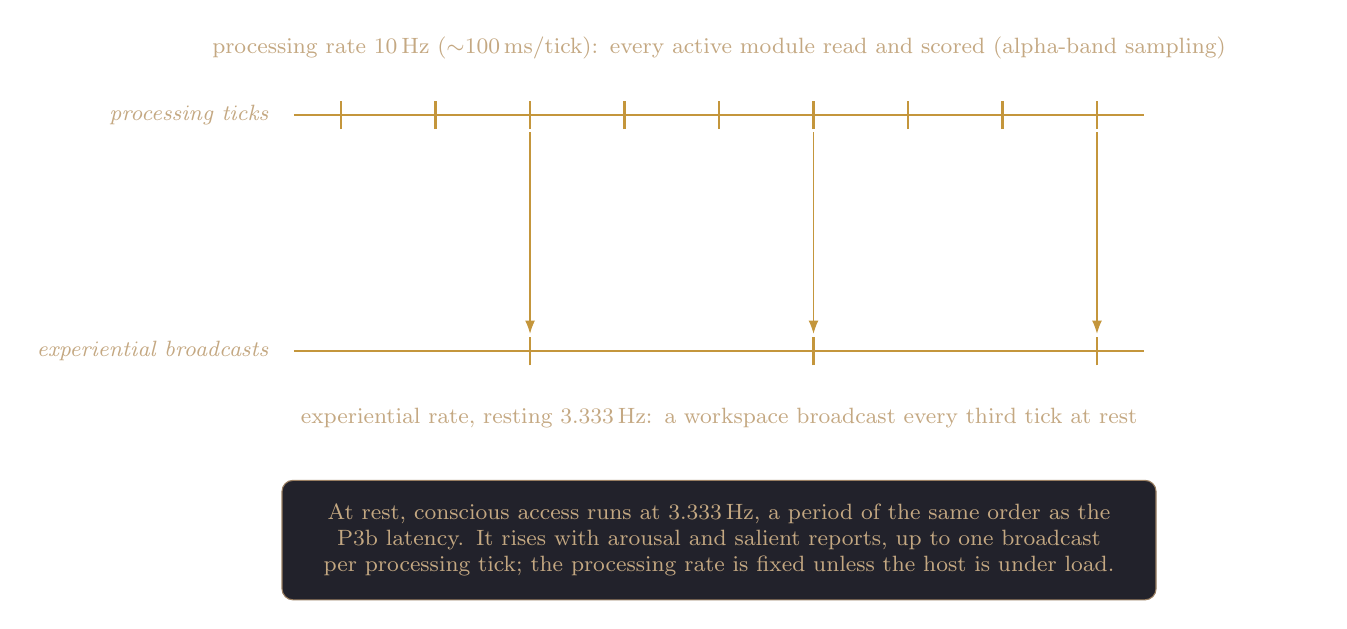
\begin{tikzpicture}[
  font=\small,>=Latex,
  every node/.append style={text=fgbody},
  every node/.append style={execute at begin node={\hyphenpenalty=10000\exhyphenpenalty=10000}},
  tickmark/.style={draw=stroke, thick},
]
\def\upy{3.0}
\def\loy{0.0}
% --- upper track: processing ticks (10 Hz) ---
\draw[thick, draw=stroke] (-0.6,\upy) -- (10.2,\upy);
\foreach \i in {0,...,8} {
  \pgfmathsetmacro{\x}{\i*1.2}
  \draw[tickmark] (\x,\upy-0.18) -- (\x,\upy+0.18);
}
\node[align=center, font=\footnotesize, text width=150mm] at (4.8,\upy+0.85)
  {processing rate 10\,Hz ($\sim$100\,ms/tick): every active module read and scored (alpha-band sampling)};
% --- lower track: experiential broadcasts (3.333 Hz) ---
\draw[thick, draw=stroke] (-0.6,\loy) -- (10.2,\loy);
\foreach \x in {2.4,6.0,9.6} {
  \draw[tickmark] (\x,\loy-0.18) -- (\x,\loy+0.18);
}
\node[align=center, font=\footnotesize, text width=120mm] at (4.8,\loy-0.85)
  {experiential rate, resting 3.333\,Hz: a workspace broadcast every third tick at rest};
% --- every third processing tick feeds a broadcast tick ---
\foreach \x in {2.4,6.0,9.6} {
  \draw[->, thin, draw=stroke] (\x,\upy-0.22) -- (\x,\loy+0.22);
}
% track labels
\node[font=\footnotesize\itshape, anchor=east] at (-0.8,\upy) {processing ticks};
\node[font=\footnotesize\itshape, anchor=east] at (-0.8,\loy) {experiential broadcasts};
% --- caption ---
\node[draw=bdim, rounded corners, fill=surf, align=center, font=\footnotesize, text width=105mm, inner sep=3mm] at (4.8,-2.4)
  {At rest, conscious access runs at 3.333\,Hz, a period of the same order as the P3b latency. It rises with arousal and salient reports, up to one broadcast per processing tick; the processing rate is fixed unless the host is under load.};
\end{tikzpicture}
\end{document}
